\begin{frame}
\frametitle{Out-of-order execution}

К сожалению, описанные подходы, как есть, не будут работать...
\begin{itemize}
  \item<2-> компилятору \emph{разрешено} переставлять инструкции:
        \begin{itemize}
          \item компилятор может делать с кодом все, что угодно, пока
                наблюдаемое поведение остается неизменным;
          \item кеширование, удаление "мертвого" кода, спекулятивные записи и
                чтения и многое другое
        \end{itemize}
  \item<3-> процессоры могут использовать оптимизации изменяющие порядок работы
        с памятью:
        \begin{itemize}
          \item store buffer - сохранение данных во временный буфер вместо
                кеша;
          \item invalidate queue - отложенный сброс линии кеша;
        \end{itemize}
\end{itemize}
\end{frame}

\begin{frame}
\frametitle{Оптимизации компилятора}

Компилятор подбирает оптимальный набор инструкций реализующий заданное
наблюдаемое поведение (осторожно C и C++):
\begin{itemize}
  \item обращения к volatile данным (чтение и запись);
  \item операции ввода/вывода (printf, scanf и тд).
\end{itemize}

\onslide<2->{Если компилятору не сообщить, то он не знает:
\begin{itemize}
  \item что переменная может модифицироваться в другом потоке;
  \item что переменную может читать другой поток;
  \item что порядок обращений к переменным важен;
\end{itemize}}
\end{frame}

\begin{frame}
\frametitle{Барьеры компилятора}

\begin{itemize}
  \item Чтобы сообщить компилятору о "побочных" эффектах работы с памятью
        нужно сделать эту память частью наблюдаемого поведения - использовать
        ключевое слово volatile;
        \begin{itemize}
          \item компилятору запрещено переставлять обращения к volatile
                данным, \emph{если они разделены точкой следования};
          \item компилятор может переставлять доступ к volatile данным с
                доступом к не volatile данным;
        \end{itemize}
\end{itemize}
\end{frame}

\begin{frame}[fragile]
\frametitle{Барьеры компиялтора}

\begin{columns}[T]
  \begin{column}{.45\linewidth}
    \begin{lstlisting}
struct some_struct {
  int a, b, c;
};

struct some_struct * volatile public;

void foo(void)
{
  struct some_struct *ptr = alloc_some_struct();

  ptr->a = 1;
  ptr->b = 2;
  ptr->c = 3;
  // need something to prevent
  // reordering
  public = ptr;
}
    \end{lstlisting}
  \end{column}
  \begin{column}{.45\linewidth}
    \begin{lstlisting}
void bar(void)
{
  while (!public);
  // and here too
  assert(public->a == 1);
  assert(public->b == 2);
  assert(public->c == 3);
}
    \end{lstlisting}
  \end{column}
\end{columns}
\end{frame}

\begin{frame}[fragile]
\frametitle{Барьеры компилятора}

Итого: volatile мало чем помогает, что делать? \\
Смотреть в документацию компилятора! Например, gcc предлагает
следующее решение:

\begin{lstlisting}
#define barrier() asm volatile ("" : : : "memory")
\end{lstlisting}
\end{frame}

\begin{frame}[fragile]
\frametitle{Барьеры компилятора}

\begin{columns}[T]
  \begin{column}{.45\linewidth}
    \begin{lstlisting}
struct some_struct {
  int a, b, c;
};

#define barrier() asm volatile ("" : : : "memory")
struct some_struct *public;

void foo(void)
{
  struct some_struct *ptr = alloc_some_struct();

  ptr->a = 1;
  ptr->b = 2;
  ptr->c = 3;
  barrier();
  public = ptr;
}
    \end{lstlisting}
  \end{column}
  \begin{column}{.45\linewidth}
    \begin{lstlisting}
void bar(void)
{
  while (!public);
  barrier();
  assert(public->a == 1);
  assert(public->b == 2);
  assert(public->c == 3);
}
    \end{lstlisting}
  \end{column}
\end{columns}
\end{frame}

\begin{frame}
\frametitle{Когерентность процессорных кешей}

\begin{figure}
  \only<1>{\centering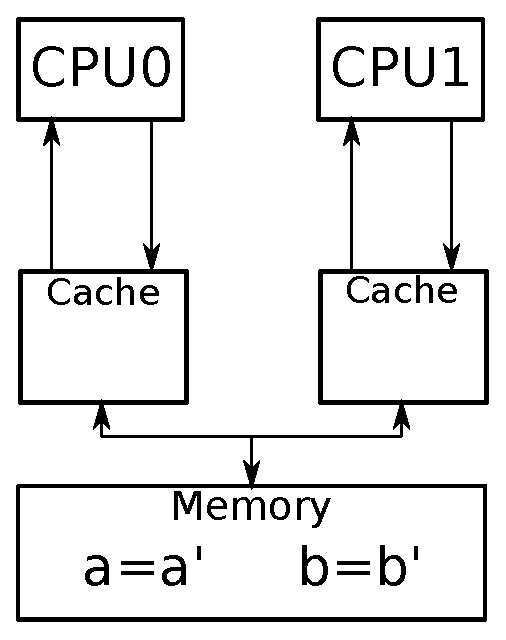
\includegraphics[height=.6\textheight]{cache-coh0}}
  \only<2>{\centering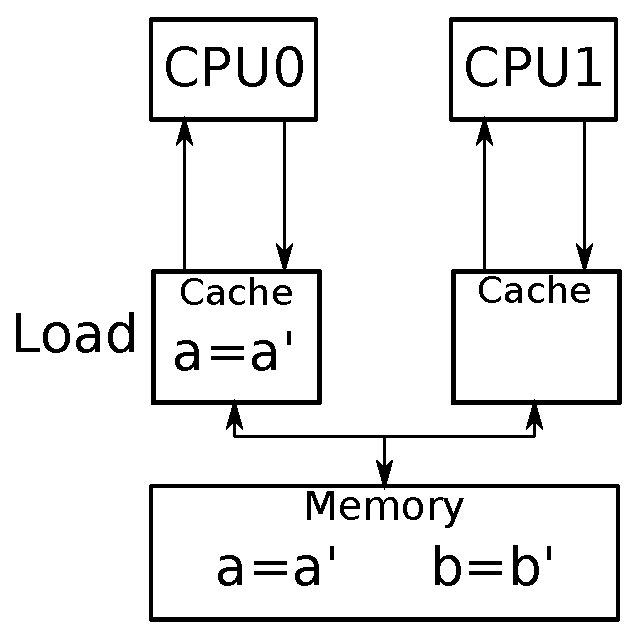
\includegraphics[height=.6\textheight]{cache-coh1}}
  \only<3>{\centering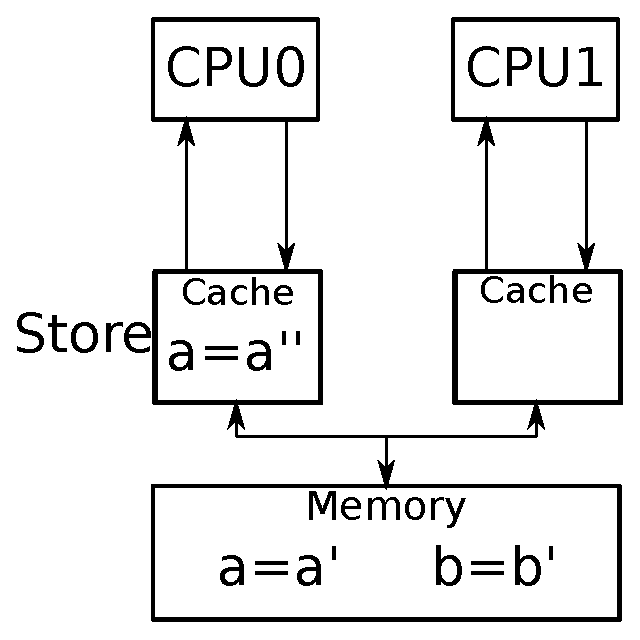
\includegraphics[height=.6\textheight]{cache-coh2}}
  \only<4>{\centering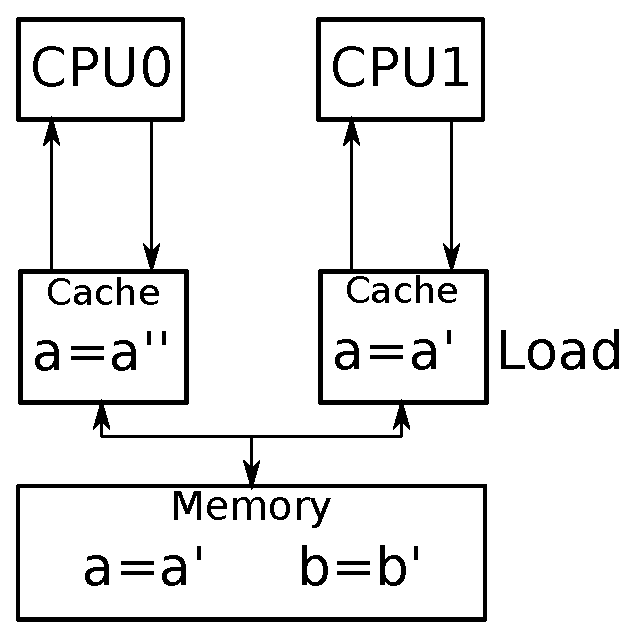
\includegraphics[height=.6\textheight]{cache-coh3}}
  \only<5>{\centering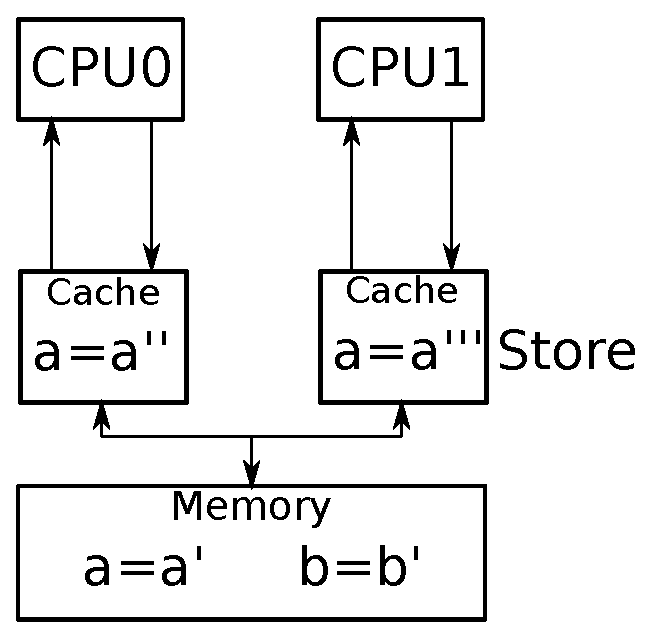
\includegraphics[height=.6\textheight]{cache-coh4}}
  \only<6>{\centering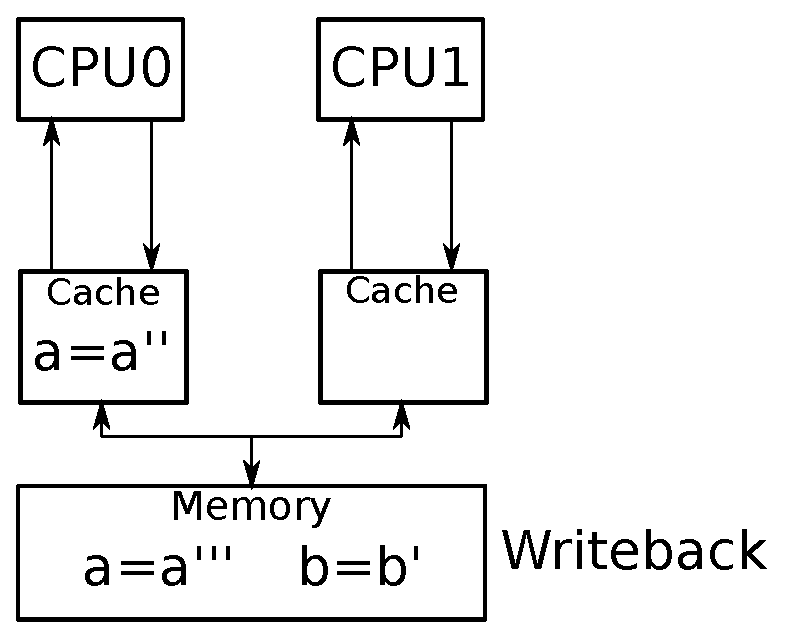
\includegraphics[height=.6\textheight]{cache-coh5}}
  \only<7>{\centering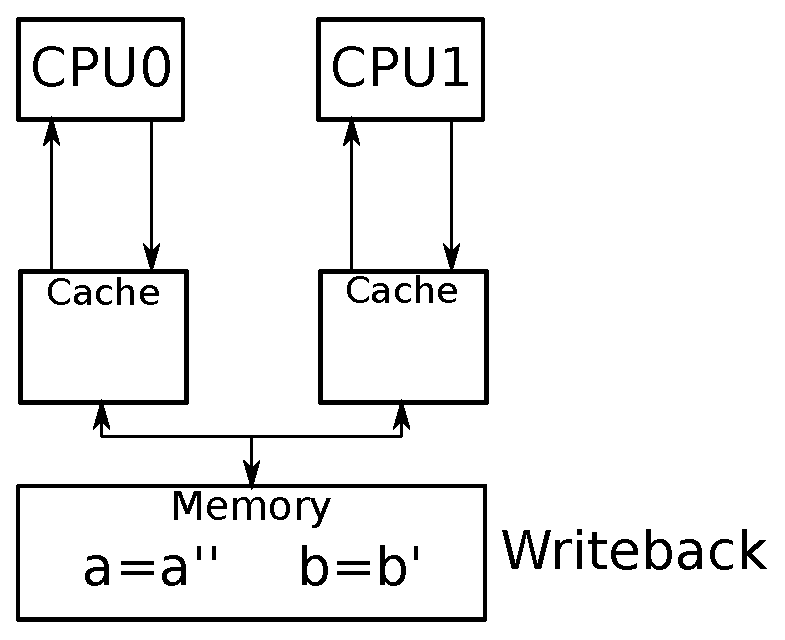
\includegraphics[height=.6\textheight]{cache-coh6}}
  \caption{Cache Incoherency}
\end{figure}
\end{frame}

\begin{frame}
\frametitle{Когерентность процессорных кешей}

Кеши должны находиться в согласованном состоянии (быть когерентными):
\begin{itemize}
  \item процессоры могут обмениваться сообщениями:
        \begin{itemize}
          \item можем считать, что сообщения передаются надежно;
          \item не можем полагаться на порядок доставки и обработки сообщений;
        \end{itemize}
  \item процессоры используют специальный протокол обеспечения когерентности:
        \begin{itemize}
          \item наверно, самый широко известный протокол - MESI (есть сомнения,
                что он используется без модификаций);
        \end{itemize}
\end{itemize}
\end{frame}

\begin{frame}
\frametitle{MESI}
MESI (Modified, Exclusive, Shared, Invalid) предполагает, что каждая линия кеша
находится в одном из четырех состояний:
\begin{itemize}
  \item Modified - кеш линия находится только в кеше данного процессора и она
        была записана (может отличаться от версии в памяти);
  \item Exclusive - кеш линия находится только в кеше данного процессора и она
        совпадает с копией в памяти;
  \item Shared - кеш линия находится в кеше данного процессора и возможно в
        кешах других процессоров, содержимое совпадает с памятью;
  \item Invalid - кеш линия не используется;
\end{itemize}
\end{frame}

\begin{frame}
\frametitle{MESI}
Перед тем как модифицировать данные процессор должен получить данные в
эксклюзивное пользование:
\begin{itemize}
  \item если несколько процессоров держат в кеше данные (Shared), то мы просим
        их сбросить данные;
  \item если другой процессор держит данные в кеше (Modified или Exclusive), то
        мы просим его передать нам данные
        \begin{itemize}
          \item контроллер памяти может увидеть передачу и обновить данные в
                памяти;
          \item или процессор может явно сбросить данные в память;
        \end{itemize}
  \item если никто не держит данные в кеше, то мы получаем их от контроллера
        памяти;
\end{itemize}
\end{frame}

\begin{frame}
\frametitle{Store Buffer}

\begin{figure}
  \centering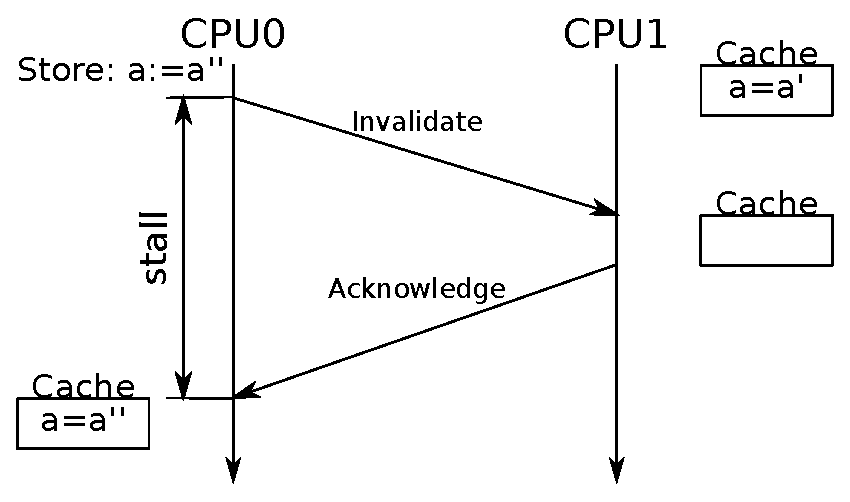
\includegraphics[width=.8\linewidth]{cache-store-stall}
  \caption{Cache Store Stall}
\end{figure}
\end{frame}

\begin{frame}
\frametitle{Store Buffer}

"Первая" запись данных приводит к ненужным остановкам конвейера:
\begin{itemize}
  \item другие процессоры должны сбросить данные из кеша;
  \item процессор должен дождаться от них подтверждения;
  \item<2-> но нам даже не нужно знать старое значение, если мы все равно его
        перезаписываем!
  \item<3-> заведем маленький кеш без поддержки когерентности (Store Buffer):
        \begin{itemize}
          \item первоначально запишем данные в него;
          \item когда придет подтверждение - сбросим данные в кеш;
        \end{itemize}
\end{itemize}
\end{frame}

\begin{frame}
\frametitle{Store Buffer}

\begin{figure}
  \centering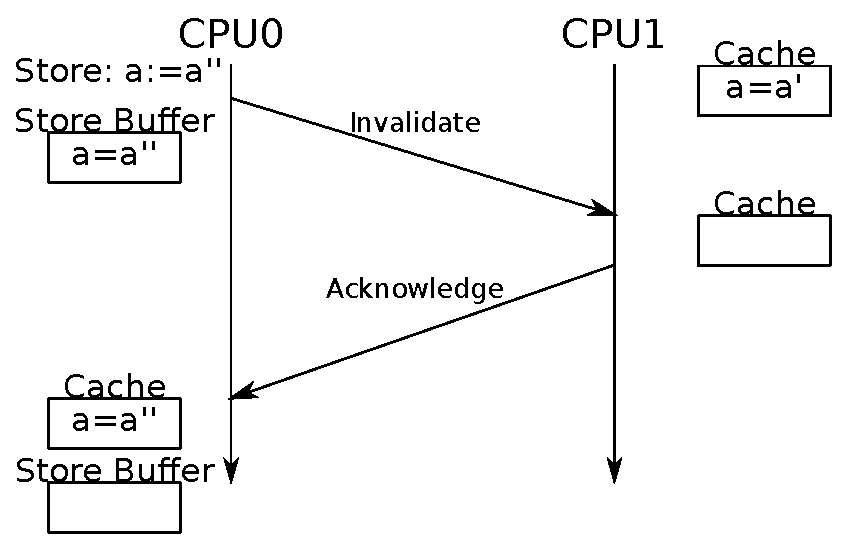
\includegraphics[width=.8\linewidth]{cache-store-buffer}
  \caption{Store Buffer}
\end{figure}
\end{frame}

\begin{frame}[fragile]
\frametitle{Memory Order Violation}

\begin{columns}[T]
  \begin{column}{.4\linewidth}
    \begin{lstlisting}
void foo(void)
{
  a = 1;
  barrier();
  b = 1;
}

void bar(void)
{
  while (b == 0)
    continue;
  barrier();
  assert(a == 1);
}
    \end{lstlisting}
  \end{column}
  \begin{column}{.6\linewidth}
    \begin{itemize}
      \item $a$ равна 0 и находится в кеше CPU1;
      \item $b$ равна 0 и находится в кеше CPU0;
      \item CPU0 исполняет foo и CPU1 исполняет bar;
    \end{itemize}
  \end{column}
\end{columns}
\end{frame}

\begin{frame}[fragile]
\frametitle{Memory Order Violation}

\begin{columns}[T]
  \begin{column}{.4\linewidth}
    \begin{lstlisting}[escapechar=!]
void foo(void)
{
  !\colorbox{hlcode}{a = 1;}!
  barrier();
  b = 1;
}

void bar(void)
{
  while (b == 0)
    continue;
  barrier();
  assert(a == 1);
}
    \end{lstlisting}
  \end{column}
  \begin{column}{.6\linewidth}
    \begin{itemize}
      \item CPU0 исполняет строку 3;
      \item переменная $a$ не в кеше CPU0 - посылаем Invalidate;
      \item сохраняем новое значение для $a$ в Store Buffer;
    \end{itemize}
  \end{column}
\end{columns}
\end{frame}

\begin{frame}[fragile]
\frametitle{Memory Order Violation}

\begin{columns}[T]
  \begin{column}{.4\linewidth}
    \begin{lstlisting}[escapechar=!]
void foo(void)
{
  a = 1;
  barrier();
  b = 1;
}

void bar(void)
{
  !\colorbox{hlcode}{while (b == 0)}!
    continue;
  barrier();
  assert(a == 1);
}
    \end{lstlisting}
  \end{column}
  \begin{column}{.6\linewidth}
    \begin{itemize}
      \item CPU1 исполняет строку 10;
      \item переменная $b$ не в кеше CPU1 - запрашиваем ее для чтения;
    \end{itemize}
  \end{column}
\end{columns}
\end{frame}

\begin{frame}[fragile]
\frametitle{Memory Order Violation}

\begin{columns}[T]
  \begin{column}{.4\linewidth}
    \begin{lstlisting}[escapechar=!]
void foo(void)
{
  a = 1;
  barrier();
  !\colorbox{hlcode}{b = 1;}!
}

void bar(void)
{
  while (b == 0)
    continue;
  barrier();
  assert(a == 1);
}
    \end{lstlisting}
  \end{column}
  \begin{column}{.6\linewidth}
    \begin{itemize}
      \item CPU0 исполняет строку 5;
      \item переменная $b$ лежит в кеше CPU0 - можно ее прям там и обновить
            (кеш линия Modified или Exclusive);
    \end{itemize}
  \end{column}
\end{columns}
\end{frame}

\begin{frame}[fragile]
\frametitle{Memory Order Violation}

\begin{columns}[T]
  \begin{column}{.4\linewidth}
    \begin{lstlisting}[escapechar=!]
void foo(void)
{
  a = 1;
  barrier();
  b = 1;
}

void bar(void)
{
  while (b == 0)
    continue;
  barrier();
  assert(a == 1);
}
    \end{lstlisting}
  \end{column}
  \begin{column}{.6\linewidth}
    \begin{itemize}
      \item CPU0 получает запрос на чтение $b$ от CPU1;
      \item CPU0 отправляет последнее значение $b = 1$;
      \item CPU0 помечает кеш линию с переменной $b$ как Shared;
    \end{itemize}
  \end{column}
\end{columns}
\end{frame}

\begin{frame}[fragile]
\frametitle{Memory Order Violation}

\begin{columns}[T]
  \begin{column}{.4\linewidth}
    \begin{lstlisting}[escapechar=!]
void foo(void)
{
  a = 1;
  barrier();
  b = 1;
}

void bar(void)
{
  !\colorbox{hlcode}{while (b == 0)}!
    continue;
  barrier();
  assert(a == 1);
}
    \end{lstlisting}
  \end{column}
  \begin{column}{.6\linewidth}
    \begin{itemize}
      \item CPU1 получает ответ от CPU0 со значением $b$;
      \item CPU1 помещает значение $b$ в кеш (кеш линия Shared);
      \item CPU1 может закончить выполнение строки 10 - условие ложно;
    \end{itemize}
  \end{column}
\end{columns}
\end{frame}

\begin{frame}[fragile]
\frametitle{Memory Order Violation}

\begin{columns}[T]
  \begin{column}{.4\linewidth}
    \begin{lstlisting}[escapechar=!]
void foo(void)
{
  a = 1;
  barrier();
  b = 1;
}

void bar(void)
{
  while (b == 0)
    continue;
  barrier();
  !\colorbox{hlcode}{assert(a == 1);}!
}
    \end{lstlisting}
  \end{column}
  \begin{column}{.6\linewidth}
    \begin{itemize}
      \item CPU1 исполняет строку 12;
      \item CPU1 держит в кеше старое значение $a = 0$;
    \end{itemize}
  \end{column}
\end{columns}
\end{frame}

\begin{frame}[fragile]
\frametitle{Memory Order Violation}

\begin{columns}[T]
  \begin{column}{.4\linewidth}
    \begin{lstlisting}[escapechar=!]
void foo(void)
{
  a = 1;
  barrier();
  b = 1;
}

void bar(void)
{
  while (b == 0)
    continue;
  barrier();
  assert(a == 1);
}
    \end{lstlisting}
  \end{column}
  \begin{column}{.6\linewidth}
    \begin{itemize}
      \item CPU1 получает Invalidate - но уже поздно;
      \item CPU1 сбрасывает линию и посылает Acknowledge CPU0;
    \end{itemize}
  \end{column}
\end{columns}
\end{frame}

\begin{frame}
\frametitle{Store Barrier}

\begin{itemize}
  \item Процессор ничего не знает о зависимостях между переменными
        \begin{itemize}
          \item он ничего не знал, о том, что сохранение $a$ должно
                предшествовать сохранению $b$;
        \end{itemize}
  \item чтобы указать процессору на зависимость используется специальная
        инструкция-барьер
        \begin{itemize}
          \item в x86 есть инструкция \emph{sfence}, которая гарантирует, что
                все записи начатые перед барьером "завершаться";
          \item другими словами \emph{sfence} ждет, пока Store Buffer опустеет;
          \item \emph{sfence} сериализует только store операции;
        \end{itemize}
\end{itemize}
\end{frame}

\begin{frame}
\frametitle{Invalidate Queue}

\begin{itemize}
  \item Store Buffer имеет ограниченный размер и может переполнится
        \begin{itemize}
          \item хочется получать Acknowledge на Invalidate побыстрее;
          \item сброс данных из кеша может занять время (если кеш занят или если
                много Invalidate сообщений пришло за раз);
        \end{itemize}
  \item процессор может отложить инвалидацию кеша и послать Acknowledge почти
        сразу
        \begin{itemize}
          \item при этом, конечно, он должен воздержаться от общения с другими
                CPU об "инвалидированной" кеш линии;
          \item Invalidate при этом ставится в очередь (CPU обращается к этой
                очереди, только если собирается послать сообщение кому-то);
        \end{itemize}
\end{itemize}
\end{frame}

\begin{frame}[fragile]
\frametitle{Memory Order Violation}

\begin{columns}[T]
  \begin{column}{.4\linewidth}
    \begin{lstlisting}[escapechar=!]
#define wmb() asm volatile ("sfence" : : : "memory")

void foo(void)
{
  a = 1;
  wmb();
  b = 1;
}

void bar(void)
{
  while (b == 0)
    continue;
  barrier();
  assert(a == 1);
}
    \end{lstlisting}
  \end{column}
  \begin{column}{.6\linewidth}
    \begin{itemize}
      \item $a = 0$ и она находится в кеше обоих процессоров (Shared);
      \item $b = 0$ и она находится в кеше CPU0 (Exclusive или Modified);
      \item CPU0 исполняет foo, а CPU1 исполняет bar;
    \end{itemize}
  \end{column}
\end{columns}
\end{frame}

\begin{frame}[fragile]
\frametitle{Memory Order Violation}

\begin{columns}[T]
  \begin{column}{.4\linewidth}
    \begin{lstlisting}[escapechar=!]
#define wmb() asm volatile ("sfence" : : : "memory")

void foo(void)
{
  !\colorbox{hlcode}{a = 1;}!
  wmb();
  b = 1;
}

void bar(void)
{
  while (b == 0)
    continue;
  barrier();
  assert(a == 1);
}
    \end{lstlisting}
  \end{column}
  \begin{column}{.6\linewidth}
    \begin{itemize}
      \item CPU0 исполняет строку 5;
      \item кеш линия помечена как Shared - нужно послать Invalidate;
    \end{itemize}
  \end{column}
\end{columns}
\end{frame}

\begin{frame}[fragile]
\frametitle{Memory Order Violation}

\begin{columns}[T]
  \begin{column}{.4\linewidth}
    \begin{lstlisting}[escapechar=!]
#define wmb() asm volatile ("sfence" : : : "memory")

void foo(void)
{
  a = 1;
  wmb();
  b = 1;
}

void bar(void)
{
  !\colorbox{hlcode}{while (b == 0)}!
    continue;
  barrier();
  assert(a == 1);
}
    \end{lstlisting}
  \end{column}
  \begin{column}{.6\linewidth}
    \begin{itemize}
      \item CPU1 исполняет строку 12;
      \item $b$ не в кеше CPU1 - запрашиваем значение $b$;
    \end{itemize}
  \end{column}
\end{columns}
\end{frame}

\begin{frame}[fragile]
\frametitle{Memory Order Violation}

\begin{columns}[T]
  \begin{column}{.4\linewidth}
    \begin{lstlisting}[escapechar=!]
#define wmb() asm volatile ("sfence" : : : "memory")

void foo(void)
{
  a = 1;
  wmb();
  b = 1;
}

void bar(void)
{
  while (b == 0)
    continue;
  barrier();
  assert(a == 1);
}
    \end{lstlisting}
  \end{column}
  \begin{column}{.6\linewidth}
    \begin{itemize}
      \item CPU1 получает Invalidate от CPU0;
      \item CPU1 сохраняет запись в Invalidate Queue, но \emph{не сбрасывает}
            кеш линию;
      \item CPU1 отправляет Acknowledge CPU0;
    \end{itemize}
  \end{column}
\end{columns}
\end{frame}

\begin{frame}[fragile]
\frametitle{Memory Order Violation}

\begin{columns}[T]
  \begin{column}{.4\linewidth}
    \begin{lstlisting}[escapechar=!]
#define wmb() asm volatile ("sfence" : : : "memory")

void foo(void)
{
  a = 1;
  !\colorbox{hlcode}{wmb();}!
  b = 1;
}

void bar(void)
{
  while (b == 0)
    continue;
  barrier();
  assert(a == 1);
}
    \end{lstlisting}
  \end{column}
  \begin{column}{.6\linewidth}
    \begin{itemize}
      \item CPU0 получает Acknowledge от CPU1;
      \item CPU0 может переместить значение $b$ из Store Buffer в кеш и может
            завершить выполнение барьера;
    \end{itemize}
  \end{column}
\end{columns}
\end{frame}

\begin{frame}[fragile]
\frametitle{Memory Order Violation}

\begin{columns}[T]
  \begin{column}{.4\linewidth}
    \begin{lstlisting}[escapechar=!]
#define wmb() asm volatile ("sfence" : : : "memory")

void foo(void)
{
  a = 1;
  wmb();
  !\colorbox{hlcode}{b = 1;}!
}

void bar(void)
{
  while (b == 0)
    continue;
  barrier();
  assert(a == 1);
}
    \end{lstlisting}
  \end{column}
  \begin{column}{.6\linewidth}
    \begin{itemize}
      \item CPU0 выполняет строку 7;
      \item $b$ уже в кеше CPU0 и CPU0 владеет этими данными - можно обновить
            прямо в кеше;
    \end{itemize}
  \end{column}
\end{columns}
\end{frame}

\begin{frame}[fragile]
\frametitle{Memory Order Violation}

\begin{columns}[T]
  \begin{column}{.4\linewidth}
    \begin{lstlisting}[escapechar=!]
#define wmb() asm volatile ("sfence" : : : "memory")

void foo(void)
{
  a = 1;
  wmb();
  b = 1;
}

void bar(void)
{
  while (b == 0)
    continue;
  barrier();
  assert(a == 1);
}
    \end{lstlisting}
  \end{column}
  \begin{column}{.6\linewidth}
    \begin{itemize}
      \item CPU0 получает запрос на чтение $b$ из CPU1;
      \item CPU0 отправляет обновленное значение $b$;
    \end{itemize}
  \end{column}
\end{columns}
\end{frame}

\begin{frame}[fragile]
\frametitle{Memory Order Violation}

\begin{columns}[T]
  \begin{column}{.4\linewidth}
    \begin{lstlisting}[escapechar=!]
#define wmb() asm volatile ("sfence" : : : "memory")

void foo(void)
{
  a = 1;
  wmb();
  b = 1;
}

void bar(void)
{
  !\colorbox{hlcode}{while (b == 0)}!
    continue;
  barrier();
  assert(a == 1);
}
    \end{lstlisting}
  \end{column}
  \begin{column}{.6\linewidth}
    \begin{itemize}
      \item CPU1 получает ответ на запрос на чтение $b$ от CPU0;
      \item CPU1 сохраняет полученное $b$ в кеш и может завершить проверку
            условия - условие ложно;
    \end{itemize}
  \end{column}
\end{columns}
\end{frame}

\begin{frame}[fragile]
\frametitle{Memory Order Violation}

\begin{columns}[T]
  \begin{column}{.4\linewidth}
    \begin{lstlisting}[escapechar=!]
#define wmb() asm volatile ("sfence" : : : "memory")

void foo(void)
{
  a = 1;
  wmb();
  b = 1;
}

void bar(void)
{
  while (b == 0)
    continue;
  barrier();
  !\colorbox{hlcode}{assert(a == 1);}!
}
    \end{lstlisting}
  \end{column}
  \begin{column}{.6\linewidth}
    \begin{itemize}
      \item CPU1 выполняет строку 15;
      \item CPU1 старое значение $a = 0$ все еще в кеше (мы не пометили ее как
            Invalid, а сразу отправили подтверждение);
    \end{itemize}
  \end{column}
\end{columns}
\end{frame}

\begin{frame}[fragile]
\frametitle{Memory Order Violation}

\begin{columns}[T]
  \begin{column}{.4\linewidth}
    \begin{lstlisting}[escapechar=!]
#define wmb() asm volatile ("sfence" : : : "memory")

void foo(void)
{
  a = 1;
  wmb();
  b = 1;
}

void bar(void)
{
  while (b == 0)
    continue;
  barrier();
  assert(a == 1);
}
    \end{lstlisting}
  \end{column}
  \begin{column}{.6\linewidth}
    \begin{itemize}
      \item CPU1 обрабатывает отложенный Invalidate, но слишком поздно;
    \end{itemize}
  \end{column}
\end{columns}
\end{frame}

\begin{frame}
\frametitle{Invalidate Queue}

\begin{itemize}
  \item Процессор ничего не знает о зависимостях между переменными
        \begin{itemize}
          \item он ничего не знал, о том, что чтение $b$ должно строго
                предшествовать чтению $a$ и "прочитал $a$" заранее;
        \end{itemize}
  \item чтобы указать процессору на зависимость используется специальная
        инструкция-барьер
        \begin{itemize}
          \item в x86 есть инструкция \emph{lfence}, которая запрещает
                переставлять операции чтения;
          \item другими словами \emph{lfence} ждет, пока Invalidate Queue
                опустеет;
        \end{itemize}
\end{itemize}
\end{frame}

\begin{frame}
\frametitle{Осторожно x86}

Важное замечание касательно примеров:
\begin{itemize}
  \item в примерах выше sfence не нужен:
        \begin{itemize}
          \item архитектура x86 гарантирует, что store операции одного
                процессора не могут быть "переставлены";
        \end{itemize}
  \item в примерах выше lfence не нужен:
        \begin{itemize}
          \item архитектура x86 гарантирует, что load операции одного
                процессора не будут переставлены друг с другом;
        \end{itemize}
\end{itemize}
\end{frame}
